\documentclass[../report.tex]{subfiles}

\begin{document}

Chức năng của hệ thống được thiết kế dựa theo những tác nhân khác nhau của hệ thống. 
Tác nhân hệ thống được chia thành 2 nhóm, với nhu cầu sử dụng khác nhau: 
\begin{itemize}
    \item Bạn đọc:
        \begin{itemize}
            \item Khách: Sử dụng thư viện chỉ với mục đích tra cứu tài liệu. 
            \item Sinh viên: Sử dụng thư viện với mục đích tra cứu tài liệu và mượn tài liệu. 
        \end{itemize}
    \item Quản lý thư viện: 
        \begin{itemize}
            \item Thủ kho: Quản lý cập nhật tài liệu mỗi khi có tài liệu mới được thêm vào hoặc tài liệu cũ muốn bỏ đi. 
            \item Giáo vụ: Xử lý thủ tục nhận trả sách cho sinh viên và biên tập nội dung tin tức trên trang chủ của hệ thống. 
        \end{itemize}
\end{itemize}

\subsection{Biểu đồ Activity}
\begin{figure}[H]
\centering
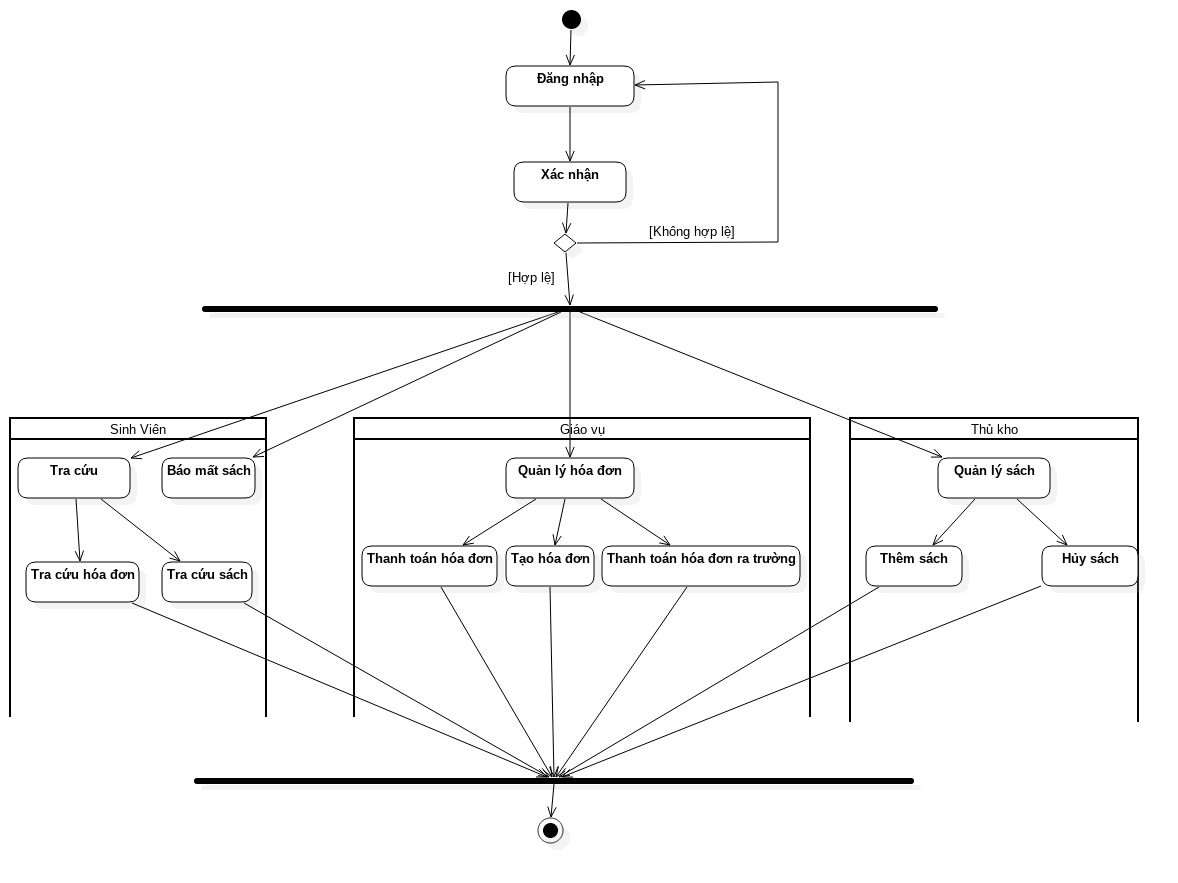
\includegraphics[width=\textwidth]{figures/active.png}
\caption{Biểu đồ hoạt động của thư viện}
\end{figure}

\begin{figure}[H]
\centering
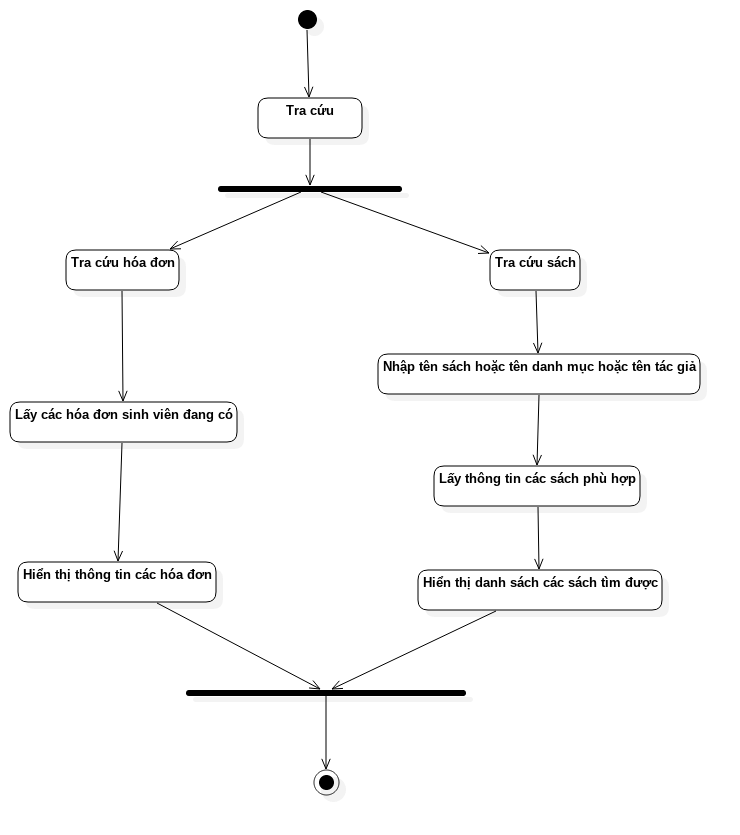
\includegraphics[width=9cm]{figures/tracuu.png}
\caption{Biểu đồ tra cứu}
\end{figure}

\begin{figure}[H]
\centering
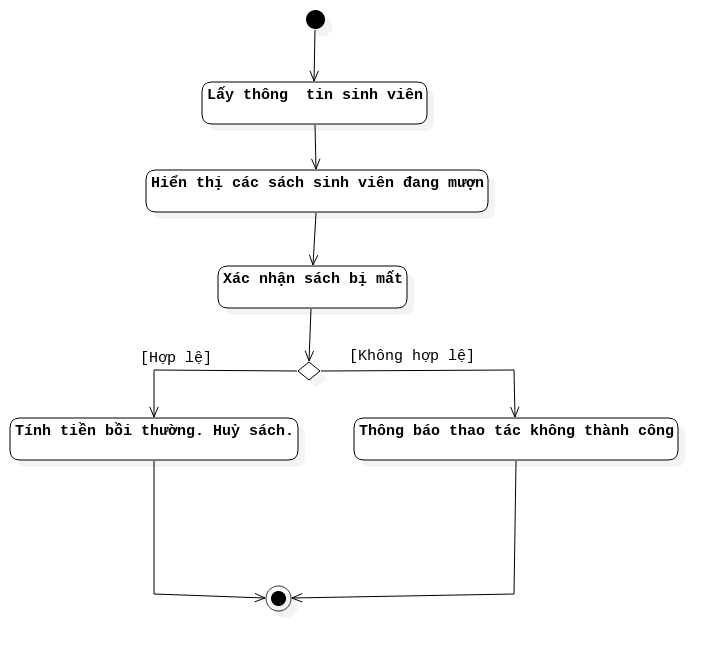
\includegraphics[width=11cm]{figures/baomatsach.png}
\caption{Biểu đồ báo mất sách}
\end{figure}

\begin{figure}[H]
\centering
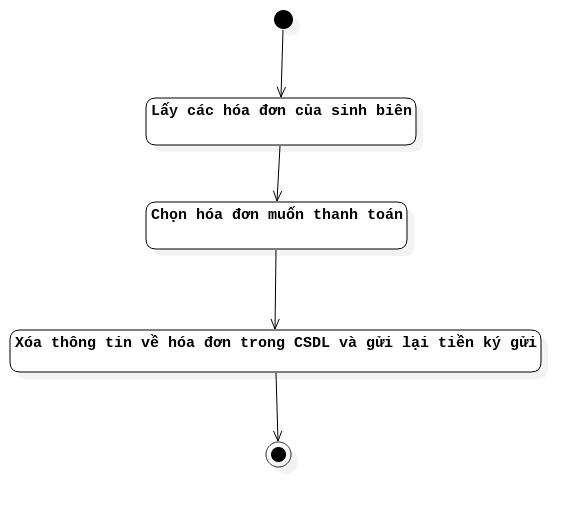
\includegraphics[width=10cm]{figures/thanhtoan.png}
\caption{Biểu đồ thanh toán hóa đơn}
\end{figure}

\begin{figure}[H]
\centering
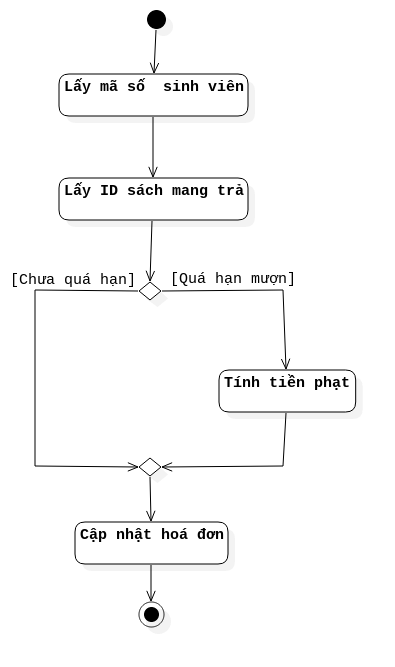
\includegraphics[width=5cm]{figures/nhantrasach.png}
\caption{Biểu đồ nhận trả sách}
\end{figure}

\begin{figure}[H]
\centering
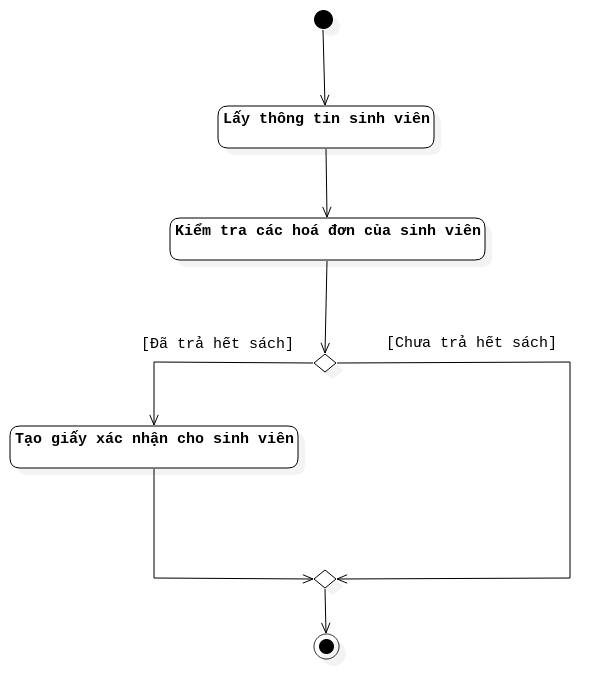
\includegraphics[width=10cm]{figures/thanhtoanratruong.png}
\caption{Biểu đồ thanh toán hóa đơn ra trường}
\end{figure}

\begin{figure}[H]
\centering
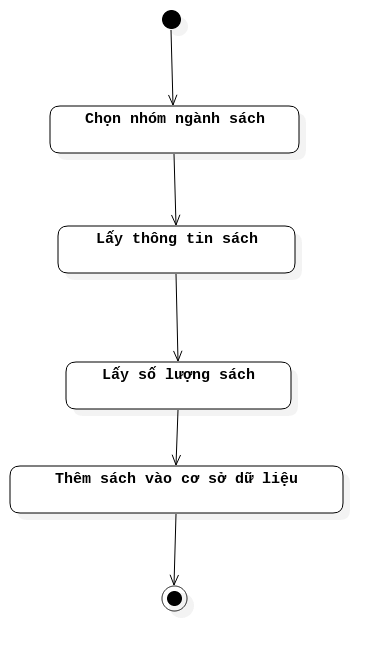
\includegraphics[width=6cm]{figures/themsach.png}
\caption{Biểu đồ thêm sách}
\end{figure}

\begin{figure}[H]
\centering
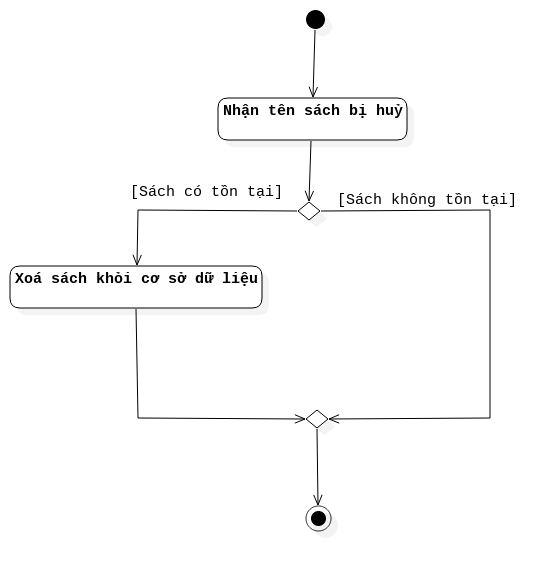
\includegraphics[width=9cm]{figures/huysach.png}
\caption{Biểu đồ hủy sách}
\end{figure}

\subsection{Đặc tả Use-Case}

\begin{center}

\newpage
\begin{tabular}{| m{6cm} | m{3cm} | m{6cm} |}
    \hline
    \textbf{Tên ca sử dụng}: Đăng nhập & \textbf{ID}: 1 & \textbf{Mức độ quan trọng}: high \\
    \hline
    \textbf{Tác nhân chính}: Khách & \multicolumn{2}{|l|}{\textbf{Loại ca sử dụng}: Chi tiết, cần thiết.} \\
    \hline
\end{tabular}
\begin{tabular}{| m{15.9cm} |}
    \hline
        \textbf{Các bên liên quan:} 
        \begin{itemize}
            \item Khách - Muốn đăng nhập để sử dụng các chức năng mà hệ thống cung cấp cho loại tài khoản User. 
            \item Sinh viên - Muốn đăng nhập để quản lý thông tin tài khoản và thông tin về hóa đơn mượn sách. 
            \item Thủ kho và Giáo vụ - Bắt buộc phải đăng nhập để có thể sử dụng được vai trò của mình trong hệ thống. 
        \end{itemize} \\
    \hline
\end{tabular}

\begin{tabular}{| m{15.9cm} |}
    \hline
    \textbf{Khởi tạo}: Khách hàng nhập thông tin về tên tài khoản và mật khẩu sau đó ấn ``Đăng nhập''. \\
    \textbf{Loại}: Bên ngoài.  \\
    \hline
\end{tabular}

\begin{tabular}{| m{15.9cm} |}
    \hline
    \textbf{Quan hệ}:
    \begin{itemize}
        \item Association: Khách, Sinh viên, Thủ kho, Giáo vụ. 
        \item Include: 
        \item Extend: 
        \item Generalization: 
    \end{itemize} \\
    \hline
\end{tabular}

\begin{tabular}{| m{15.9cm} |}
    \hline
    \textbf{Luồng sự kiện chính}:
    \begin{enumerate}
        \item Lựa chọn chức năng đăng nhập. 
        \item Nhập tên tài khoản và mật khẩu. 
        \item Hệ thống xác thực thông tin nhập vào: 
        \begin{enumerate}
            \item Nếu đúng: Thông báo đăng nhập thành công, trả về giao diện ứng với quyền truy cập của tài khoản đăng nhập. 
            \item nếu sai: Thông báo người dùng nhập bị sai và yêu cầu nhập lại. 
        \end{enumerate}
    \end{enumerate} \\
    \hline
\end{tabular}

\begin{tabular}{| m{15.9cm} |}
    \hline
    \textbf{Luồng ngoại lệ}:
    \begin{enumerate}
        \item[3.b] Người dùng lựa chọn ``Quên mật khẩu'' khi không nhớ chính xác mật khẩu của tài khoản hiện tại và muốn đặt lại mật khẩu cho tài khoản. 
    \end{enumerate} \\
    \hline
\end{tabular}

\newpage
\begin{tabular}{| m{6cm} | m{3cm} | m{6cm} |}
    \hline
    \textbf{Tên ca sử dụng}: Tra cứu sách & \textbf{ID}: 2 & \textbf{Mức độ quan trọng}: high \\
    \hline
    \textbf{Tác nhân chính}: Khách, Sinh viên, Thủ kho, Giáo vụ & \multicolumn{2}{|l|}{\textbf{Loại ca sử dụng}: Đơn giản, cần thiết.} \\
    \hline
\end{tabular}
\begin{tabular}{| m{15.9cm} |}
    \hline
        \textbf{Các bên liên quan:} 
        \begin{itemize}
            \item Khách - Muốn tìm kiếm sách trong tập dữ liệu sách đang có trong thư viện. 
            \item Sinh viên - Muốn tra cứu sách để mượn về hoặc đọc tại thư viện. 
            \item Thủ kho - Muốn có thông tin về các sách hiện có trong thư viện để có thể điều chỉnh lượng sách trong các phòng ban cho cân bằng. 
            \item Giáo vụ - Muốn có thông tin sách để biên tập nội dung tin tức trên trang chủ của thư viện. 
        \end{itemize} \\
    \hline
\end{tabular}

\begin{tabular}{| m{15.9cm} |}
    \hline
    \textbf{Khởi tạo}: Khách, Sinh viên, Thủ kho, Giáo vụ phòng mượn \\
    \textbf{Loại}: Bên ngoài.  \\
    \hline
\end{tabular}

\begin{tabular}{| m{15.9cm} |}
    \hline
    \textbf{Quan hệ}:
    \begin{itemize}
        \item Association: Khách, Sinh viên, Thủ kho, Giáo vụ. 
        \item Include: 
        \item Extend: 
        \item Generalization: 
    \end{itemize} \\
    \hline
\end{tabular}

\begin{tabular}{| m{15.9cm} |}
    \hline
    \textbf{Luồng sự kiện chính}:
    \begin{enumerate}
        \item Nhập thông tin về sách cần tìm: Có thể tìm sách theo tên hoặc theo danh mục hoặc theo tác giả. 
        \item Trả về kết quả tìm kiếm. 
    \end{enumerate} \\
    \hline
\end{tabular}

\begin{tabular}{| m{15.9cm} |}
    \hline
    \textbf{Luồng ngoại lệ}: Khi có được kết quả tìm kiếm, bạn đọc có thể lọc sách cần tìm theo tên / NXB / tác giả. \\
    \hline
\end{tabular}

\newpage
\begin{tabular}{| m{6cm} | m{3cm} | m{6cm} |}
    \hline
    \textbf{Tên ca sử dụng}: Tra cứu hóa đơn & \textbf{ID}: 3 & \textbf{Mức độ quan trọng}: medium \\
    \hline
    \textbf{Tác nhân chính}: Sinh viên, Giáo vụ & \multicolumn{2}{|l|}{\textbf{Loại ca sử dụng}: Cơ bản, cần thiết.} \\
    \hline
\end{tabular}
\begin{tabular}{| m{15.9cm} |}
    \hline
        \textbf{Các bên liên quan:} 
        \begin{itemize}
            \item Sinh viên - Muốn xem thông tin về hóa đơn mượn sách tính tới thời điểm hiện tại. 
            \item Giáo vụ - Cần thông tin từ hóa đơn để có thể thanh toán hóa đơn cho sinh viên muốn trả lại các sách đã mượn. 
        \end{itemize} \\
    \hline
\end{tabular}

\begin{tabular}{| m{15.9cm} |}
    \hline
    \textbf{Khởi tạo}: Sinh viên yêu cầu xem thông tin về hóa đơn thông qua chức năng tra cứu hóa đơn của hệ thống. \\
    \textbf{Loại}: Bên ngoài.  \\
    \hline
\end{tabular}

\begin{tabular}{| m{15.9cm} |}
    \hline
    \textbf{Quan hệ}:
    \begin{itemize}
        \item Association: Sinh viên, Giáo vụ. 
        \item Include: 
        \item Extend: 
        \item Generalization: 
    \end{itemize} \\
    \hline
\end{tabular}

\begin{tabular}{| m{15.9cm} |}
    \hline
    \textbf{Luồng sự kiện chính}:
    \begin{enumerate}
        \item Sinh viên / Giáo vụ đăng nhập hệ thống. 
        \item Lựa chọn chức năng ``Tra cứu hóa đơn'' trên giao diện của hệ thống. 
        \item Hệ thống trả lại thông tin các hóa đơn chưa hoàn tất thanh toán ứng với MSSV được cung cấp. 
    \end{enumerate} \\
    \hline
\end{tabular}

\newpage
\begin{tabular}{| m{6cm} | m{3cm} | m{6cm} |}
    \hline
    \textbf{Tên ca sử dụng}: Báo mất sách & \textbf{ID}: 4 & \textbf{Mức độ quan trọng}: medium \\
    \hline
    \textbf{Tác nhân chính}: Sinh viên & \multicolumn{2}{|l|}{\textbf{Loại ca sử dụng}: Đơn giản, cần thiết.} \\
    \hline
\end{tabular}
\begin{tabular}{| m{15.9cm} |}
    \hline
        \textbf{Các bên liên quan:} 
        \begin{itemize}
            \item Sinh viên - thông báo bị mất sách để được xử lý. 
        \end{itemize} \\
    \hline
\end{tabular}

\begin{tabular}{| m{15.9cm} |}
    \hline
    \textbf{Khởi tạo}: Sinh viên thông báo mất sách với hệ thống. \\
    \textbf{Loại}: Bên trong.  \\
    \hline
\end{tabular}

\begin{tabular}{| m{15.9cm} |}
    \hline
    \textbf{Quan hệ}:
    \begin{itemize}
        \item Association: Sinh viên.
        \item Include: 
        \item Extend: 
        \item Generalization: 
    \end{itemize} \\
    \hline
\end{tabular}

\begin{tabular}{| m{15.9cm} |}
    \hline
    \textbf{Luồng sự kiện chính}:
    \begin{enumerate}
        \item Sinh viên đăng nhập và lựa chọn báo mất sách. 
        \item Hệ thống trả về thông tin các sách đang mượn.
        \item Chọn sách bị mất.
        \item Hệ thống kiểm tra thông tin sách bị mất, khi đó:
        \begin{enumerate}
            \item Nếu hợp lệ (sách đã được mượn): Xóa thông tin của sách và thông báo số tiền nộp phạt.
            \item nếu không hợp lệ (sách chưa được mượn): thông báo thao tác không thành công. 
        \end{enumerate}
    \end{enumerate} \\
    \hline
\end{tabular}

\newpage
\begin{tabular}{| m{6cm} | m{3cm} | m{6cm} |}
    \hline
    \textbf{Tên ca sử dụng}: Tạo hóa đơn & \textbf{ID}: 5 & \textbf{Mức độ quan trọng}: high \\
    \hline
    \textbf{Tác nhân chính}: Giáo vụ  & \multicolumn{2}{|l|}{\textbf{Loại ca sử dụng}: Chi tiết, cần thiết.} \\
    \hline
\end{tabular}
\begin{tabular}{| m{15.9cm} |}
    \hline
        \textbf{Các bên liên quan:} 
        \begin{itemize}
            \item Sinh viên - Muốn mượn sách của thư viện. 
            \item Giáo vụ - Xuất hóa đơn cho sinh viên mượn sách. 
        \end{itemize} \\
    \hline
\end{tabular}

\begin{tabular}{| m{15.9cm} |}
    \hline
    \textbf{Khởi tạo}: Sinh viên mượn sách và cung cấp thông tin cho giáo vụ nhập vào hóa đơn. \\
    \textbf{Loại}: Bên ngoài.  \\
    \hline
\end{tabular}

\begin{tabular}{| m{15.9cm} |}
    \hline
    \textbf{Quan hệ}:
    \begin{itemize}
        \item Association: Giáo vụ. 
        \item Include: 
        \item Extend: 
        \item Generalization: 
    \end{itemize} \\
    \hline
\end{tabular}

\begin{tabular}{| m{15.9cm} |}
    \hline
    \textbf{Luồng sự kiện chính}:
    \begin{enumerate}
        \item Sinh viên chọn những sách cần mượn tại phòng mượn. 
        \item Mang sách tới bàn thanh toán. 
        \item Nhập vào thông tin cá nhân bao gồm: Tên, MSSV. 
        \item Giáo vụ thêm thông tin về sách được mượn vào trong hóa đơn: Mã sách, giá. 
        \item Xuất hóa đơn cho sinh viên. 
    \end{enumerate} \\
    \hline
\end{tabular}

\newpage
\begin{tabular}{| m{6cm} | m{3cm} | m{6cm} |}
    \hline
    \textbf{Tên ca sử dụng}: Thanh toán hóa đơn & \textbf{ID}: 6 & \textbf{Mức độ quan trọng}: high \\
    \hline
    \textbf{Tác nhân chính}: Giáo vụ & \multicolumn{2}{|l|}{\textbf{Loại ca sử dụng}: Đơn giản, cần thiết.} \\
    \hline
\end{tabular}
\begin{tabular}{| m{15.9cm} |}
    \hline
        \textbf{Các bên liên quan:} 
        \begin{itemize}
            \item Sinh viên - Muốn hoàn tất thanh toán hóa đơn và nhận lại tiền cọc. 
            \item Giáo vụ - Tiếp nhận và kiểm tra hóa đơn, gửi tiền cọc cho sinh viên nếu việc kiểm tra là hợp lệ. 
        \end{itemize} \\
    \hline
\end{tabular}

\begin{tabular}{| m{15.9cm} |}
    \hline
    \textbf{Khởi tạo}: Sinh viên mang hóa đơn đến gặp giáo vụ, yêu cầu thanh toán hóa đơn. \\
    \textbf{Loại}: Bên ngoài.  \\
    \hline
\end{tabular}

\begin{tabular}{| m{15.9cm} |}
    \hline
    \textbf{Quan hệ}:
    \begin{itemize}
        \item Association: Giáo vụ. 
        \item Include: 
        \item Extend: 
        \item Generalization: 
    \end{itemize} \\
    \hline
\end{tabular}

\begin{tabular}{| m{15.9cm} |}
    \hline
    \textbf{Luồng sự kiện chính}:
    \begin{enumerate}
        \item Sinh viên mang hóa đơn đến gặp giáo vụ, yêu cầu thanh toán tiền. 
        \item Giáo vụ tiếp nhận hóa đơn và nhập MSSV. 
        \item Hệ thống tìm kiếm thông tin về các hóa đơn chưa thanh toán của sinh viên. 
        \item Giáo vụ chọn hóa đơn cần thanh toán. 
        \item Hệ thống thông báo các sách chưa được trả trong hóa đơn. 
        \item Sinh viên trả sách và nhận lại số tiền đã ký gửi. 
    \end{enumerate} \\
    \hline
\end{tabular}

\begin{tabular}{| m{15.9cm} |}
    \hline
    \textbf{Luồng ngoại lệ}:
    \begin{enumerate}
        \item Sinh viên chưa trả đủ sách tương ứng với hóa đơn sẽ không được thanh toán. 
        \item Hóa đơn bị rách, tẩy xóa cũng sẽ không được thanh toán. 
    \end{enumerate} \\
    \hline
\end{tabular}

\newpage
\begin{tabular}{| m{6cm} | m{3cm} | m{6cm} |}
    \hline
    \textbf{Tên ca sử dụng}: Nhận trả sách & \textbf{ID}: 7 & \textbf{Mức độ quan trọng}: high \\
    \hline
    \textbf{Tác nhân chính}: Giáo vụ  & \multicolumn{2}{|l|}{\textbf{Loại ca sử dụng}: Đơn giản, cần thiết.} \\
    \hline
\end{tabular}
\begin{tabular}{| m{15.9cm} |}
    \hline
        \textbf{Các bên liên quan:} 
        \begin{itemize}
            \item Sinh viên - Trả lại sách đã mượn. 
            \item Giáo vụ - Cập nhật thông tin về sách được trả lại. 
        \end{itemize} \\
    \hline
\end{tabular}

\begin{tabular}{| m{15.9cm} |}
    \hline
    \textbf{Khởi tạo}: Sinh viên thông báo với giáo vụ về sách muốn trả lại. \\
    \textbf{Loại}: Bên ngoài.  \\
    \hline
\end{tabular}

\begin{tabular}{| m{15.9cm} |}
    \hline
    \textbf{Quan hệ}:
    \begin{itemize}
        \item Association: Giáo vụ. 
        \item Include: 
        \item Extend: 
        \item Generalization: 
    \end{itemize} \\
    \hline
\end{tabular}

\begin{tabular}{| m{15.9cm} |}
    \hline
    \textbf{Luồng sự kiện chính}:
    \begin{enumerate}
        \item Sinh viên thông báo với giáo vụ về sách muốn trả lại. 
        \item Giáo vụ tiếp nhận sách và nhập ID sách được trả và lựa chọn xác nhận trả sách. 
        \item Hệ thống cập nhật lại thông tin của sách được trả lại, thông báo trả sách thành công. 
    \end{enumerate} \\
    \hline
\end{tabular}

\begin{tabular}{| m{15.9cm} |}
    \hline
    \textbf{Luồng ngoại lệ}:
    \begin{enumerate}
        \item Sinh viên làm hỏng sách sẽ phải nộp tiền bồi thường. 
        \item Sinh viên trả sách quá hạn sẽ phải nộp phạt. 
    \end{enumerate} \\
    \hline
\end{tabular}

\newpage
\begin{tabular}{| m{6cm} | m{3cm} | m{6cm} |}
    \hline
    \textbf{Tên ca sử dụng}: Thanh toán & \textbf{ID}: 8 & \textbf{Mức độ quan trọng}: medium \\
    \hline
    \textbf{Tác nhân chính}: Giáo vụ  & \multicolumn{2}{|l|}{\textbf{Loại ca sử dụng}: Đơn giản, cần thiết.} \\
    \hline
\end{tabular}
\begin{tabular}{| m{15.9cm} |}
    \hline
        \textbf{Các bên liên quan:} 
        \begin{itemize}
            \item Sinh viên - Muốn xin giấy xác thực của sinh viên. 
            \item Giáo vụ - Kiểm tra và tạo giấy xác thực cho sinh viên. 
        \end{itemize} \\
    \hline
\end{tabular}

\begin{tabular}{| m{15.9cm} |}
    \hline
    \textbf{Khởi tạo}: Sinh viên đến gặp giáo vụ yêu cầu tạo giấy xác nhận của thư viện. 
    \textbf{Loại}: Bên ngoài.  \\
    \hline
\end{tabular}

\begin{tabular}{| m{15.9cm} |}
    \hline
    \textbf{Quan hệ}:
    \begin{itemize}
        \item Association: Giáo vụ. 
        \item Include: 
        \item Extend: 
        \item Generalization: 
    \end{itemize} \\
    \hline
\end{tabular}

\begin{tabular}{| m{15.9cm} |}
    \hline
    \textbf{Luồng sự kiện chính}:
    \begin{enumerate}
        \item Sinh viên đến gặp giáo vụ yêu cầu tạo giấy xác nhận của thư viện và cung cấp MSSV. 
        \item Giáo vụ nhập MSSV để kiểm tra thông tin các hóa đơn hiện có của sinh viên. 
        \item Hệ thống trả lại thông tin về các hóa đơn chưa hoàn tất thanh toán của sinh viên. 
        \item Hệ thống xóa đi tài khoản của sinh viên. 
        \item Giáo vụ phòng mượn tạo giấy xác thực của thư viện cấp cho sinh viên. 
    \end{enumerate} \\
    \hline
\end{tabular}

\begin{tabular}{| m{15.9cm} |}
    \hline
    \textbf{Luồng ngoại lệ}:
    \begin{enumerate}
        \item[3.a] Nếu không còn hóa đơn: Hệ thống trả lại biên lai xác nhận đã thanh toán. 
        \item[3.b] Nếu còn hoá đơn: Hệ thống tín toán số tiền các hóa đơn, yêu cầu thanh toán tiền. Khi sinh viên đã hoàn tất thanh toán thì sẽ 
            trả lại biên lai xác nhận đã thanh toán. 
    \end{enumerate} \\
    \hline
\end{tabular}

\newpage
\begin{tabular}{| m{6cm} | m{3cm} | m{6cm} |}
    \hline
    \textbf{Tên ca sử dụng}: Thêm sách mới & \textbf{ID}: 9 & \textbf{Mức độ quan trọng}: medium \\
    \hline
    \textbf{Tác nhân chính}: Thủ kho & \multicolumn{2}{|l|}{\textbf{Loại ca sử dụng}: Đơn giản, cần thiết.} \\
    \hline
\end{tabular}
\begin{tabular}{| m{15.9cm} |}
    \hline
        \textbf{Các bên liên quan:} 
        \begin{itemize}
            \item Thủ kho - Tiếp nhận sách, nhập thông tin sách vào CSDL. 
        \end{itemize} \\
    \hline
\end{tabular}

\begin{tabular}{| m{15.9cm} |}
    \hline
    \textbf{Khởi tạo}: Thủ kho tiếp nhận sách mới và nhập thông tin vào CSDL. \\
    \textbf{Loại}: Bên ngoài.  \\
    \hline
\end{tabular}

\begin{tabular}{| m{15.9cm} |}
    \hline
    \textbf{Quan hệ}:
    \begin{itemize}
        \item Association: Thủ kho. 
        \item Include: 
        \item Extend: 
        \item Generalization: 
    \end{itemize} \\
    \hline
\end{tabular}

\begin{tabular}{| m{15.9cm} |}
    \hline
    \textbf{Luồng sự kiện chính}:
    \begin{enumerate}
        \item Thủ kho lựa chọn chức năng thêm sách mới. 
        \item Lựa chọn nhóm ngành sách. 
        \item Nhập thông tin sách: Tên, tác giả, nhà xuất bản, năm xuất bản, giá. 
        \item Nhập số lượng sách cần thêm. 
        \item Xác nhận thêm sách. 
        \item Hệ thống tự động sinh mã sách theo thông tin vừa nhập vào. 
        \item Xác nhận thao tác thêm sách thành công. 
    \end{enumerate} \\
    \hline
\end{tabular}

\newpage
\begin{tabular}{| m{6cm} | m{3cm} | m{6cm} |}
    \hline
    \textbf{Tên ca sử dụng}: Hủy sách & \textbf{ID}: 10 & \textbf{Mức độ quan trọng}: medium \\
    \hline
    \textbf{Tác nhân chính}: Thủ kho  & \multicolumn{2}{|l|}{\textbf{Loại ca sử dụng}: Đơn giản} \\
    \hline
\end{tabular}
\begin{tabular}{| m{15.9cm} |}
    \hline
        \textbf{Các bên liên quan:} 
        \begin{itemize}
            \item Thủ kho - Loại bỏ sách cũ hỏng khỏi CSDL. 
        \end{itemize} \\
    \hline
\end{tabular}

\begin{tabular}{| m{15.9cm} |}
    \hline
    \textbf{Khởi tạo}: Thủ kho tiếp nhận thông tin về những sách cần hủy. \\
    \textbf{Loại}: Bên ngoài.  \\
    \hline
\end{tabular}

\begin{tabular}{| m{15.9cm} |}
    \hline
    \textbf{Quan hệ}:
    \begin{itemize}
        \item Association: Thủ kho. 
        \item Include: 
        \item Extend: 
        \item Generalization: 
    \end{itemize} \\
    \hline
\end{tabular}

\begin{tabular}{| m{15.9cm} |}
    \hline
    \textbf{Luồng sự kiện chính}:
    \begin{enumerate}
        \item Thủ kho tiếp nhận thông tin về những sách cần bỏ. 
        \item Nhập vào các ID sách muốn bỏ. 
        \item Hệ thống xóa thông tin của các sách muốn hủy bỏ dựa trên ID được cung cấp. 
        \item Hệ thống thông báo thao tác thành công. 
    \end{enumerate} \\
    \hline
\end{tabular}

\end{center}

\subsection{Biểu đồ Use-Case}
\begin{figure}[H]
\centering
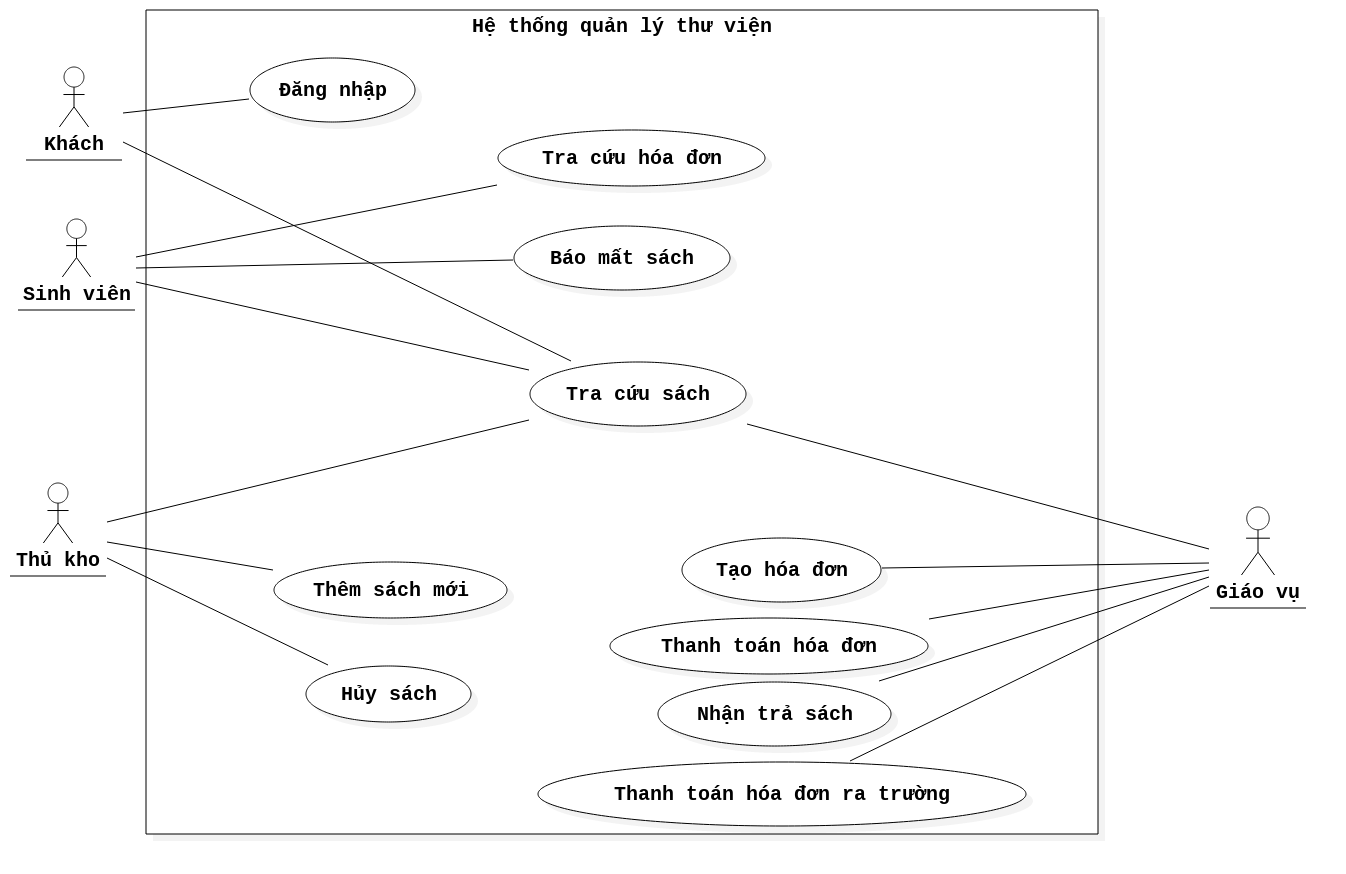
\includegraphics[width=\textwidth]{figures/usecase.png}
\caption{Biểu đồ Use-Case}
\end{figure}

\end{document}
